% main.tex — entry point for the article PDF.
% Compile (Stage 9.4+, from latex_project/):
%   xelatex -interaction=nonstopmode -halt-on-error -output-directory=build main.tex
%   biber build/main
%   xelatex ... (twice more for ToC and citations)
% Source of truth for all content: content/book.md (cleaned Markdown, immutable).

\documentclass[11pt,a4paper]{report}

% preamble.tex — packages, fonts, languages, headers/footers, bibliography.
% Engine: XeLaTeX (D-030). LuaLaTeX is the recorded fallback.
% Package order matters:
%   - fontspec before polyglossia;
%   - hyperref near the end (but before biblatex, which detects it);
%   - polyglossia + Hebrew LAST, because it loads bidi, which must load last.

% --- Page geometry (A4, ~2.5 cm margins; sized for the 13-17 page target) ---
\usepackage[a4paper,margin=2.5cm]{geometry}

% --- Fonts (XeLaTeX/fontspec; Unicode input) -------------------------------
\usepackage{fontspec}
% Latin Modern (default) for English text; DejaVu Sans for Hebrew below.
% DejaVu Sans availability was verified with fc-match before this was written.

% --- Core packages (minimal, stable set) -----------------------------------
\usepackage{graphicx}   % figures (architecture diagram + generated graph, Stage 9.2)
\usepackage{booktabs}   % tables 4.1 and 6.1
\usepackage{amsmath}    % the two numbered equations
\usepackage{xcolor}     % link colors only

% --- Headers and footers (real implementation, not conceptual) -------------
\usepackage{fancyhdr}
\pagestyle{fancy}
\fancyhf{}
\fancyhead[L]{\small From PoC to Production}
\fancyhead[R]{\small MaRs-777}
\fancyfoot[C]{\thepage}
\renewcommand{\headrulewidth}{0.4pt}
% Chapter-opening pages fall back to "plain" (page number only), as usual.

% --- Hyperlinks -------------------------------------------------------------
\usepackage[colorlinks=true,linkcolor=blue!50!black,citecolor=blue!50!black,urlcolor=blue!50!black]{hyperref}

% --- Bibliography: biblatex + biber, numeric style, linked citations -------
\usepackage[backend=biber,style=numeric,sorting=nyt]{biblatex}
\addbibresource{references.bib}

% --- Languages: English main, Hebrew other (loads bidi under XeTeX) --------
% Kept last on purpose (bidi wants to be the last loaded package).
\usepackage{polyglossia}
\setmainlanguage{english}
\setotherlanguage{hebrew}
\newfontfamily\hebrewfont[Script=Hebrew]{DejaVu Sans}


\begin{document}

% --- Cover page (mandatory PDF element) ------------------------------------
\begin{titlepage}
  \centering
  \vspace*{2cm}
  {\LARGE\bfseries From PoC to Production:\\[0.4em]
   A CrewAI Multi-Agent Pipeline for Generating a \LaTeX{} Book\par}
  \vspace{2cm}
  {\large Group: MaRs-777\par}
  \vspace{0.8cm}
  {\large Mohamed Awad \quad\textbullet\quad Rawey Sleiman\par}
  \vspace{2cm}
  {\large AI Agents / Vibe Coding course project\par}
  \vspace{0.4cm}
  {\large Lecturer contact: \href{mailto:rmisegal@gmail.com}{rmisegal@gmail.com}\par}
  \vfill
  {\large June 11, 2026\par}
\end{titlepage}

% --- Abstract ---------------------------------------------------------------
% 00_abstract.tex — skeleton. Source: content/book.md, "Abstract".
% TODO (Stage 9.3): transcribe the full abstract from content/book.md.

\chapter*{Abstract}
\addcontentsline{toc}{chapter}{Abstract}

% Placeholder summary sentence (abridged from the cleaned source; the full
% abstract is transcribed in Stage 9.3):
This report describes a CrewAI-based multi-agent pipeline for generating the
content of a \LaTeX{} book, and our experience moving it from an early
proof-of-concept toward production.


% --- Table of contents (generated automatically; no manual page numbers) ---
\tableofcontents

% --- Chapters ---------------------------------------------------------------
% 01_introduction.tex — skeleton. Source: content/book.md, "1. Introduction".
% TODO (Stage 9.3): transcribe sections 1.1-1.3 from content/book.md.

\chapter{Introduction}

\section{The Challenge of Automated Document Generation}
% TODO (Stage 9.3): content from book.md section 1.1.

\section{The Promise of Multi-Agent Systems in AI}
% TODO (Stage 9.3): content from book.md section 1.2.

\section{Project Scope and Objectives}
% TODO (Stage 9.3): content from book.md section 1.3 (objectives list).

% 02_background.tex — skeleton. Source: content/book.md, "2. Background and
% Related Work". Citation commands below mirror the [n] markers already
% present in the cleaned Markdown (sections 2.1-2.3).
% TODO (Stage 9.3): transcribe full section text from content/book.md.

\chapter{Background and Related Work}

\section{Understanding CrewAI and Multi-Agent Orchestration}
% TODO (Stage 9.3): content from book.md section 2.1.
CrewAI is an open-source framework for building and managing multi-agent
systems~\cite{crewai_docs}; the underlying idea is well established in the AI
literature~\cite{wooldridge2009mas,russell2020aima}.

\section{LaTeX: A Strong Standard for Technical Publishing}
% TODO (Stage 9.3): content from book.md section 2.2.
\LaTeX{} is a document-preparation system known for high-quality typesetting
of scientific and technical material~\cite{lamport1994latex}.

\section{Generative AI Approaches to Document Creation}
% TODO (Stage 9.3): content from book.md section 2.3.
Benchmarks such as AgentBench evaluate large language models acting as
agents~\cite{agentbench2023}.

% 03_architecture.tex — skeleton. Source: content/book.md, "3. System Design
% and Architecture".
% TODO (Stage 9.3): transcribe sections 3.1-3.3 from content/book.md.

\chapter{System Design and Architecture}

\section{Overall Pipeline Architecture}
% TODO (Stage 9.3): content from book.md section 3.1.
% TODO (Stage 9.2): architecture diagram figure. The image file does not exist
% yet, so the figure block stays commented out until figures/architecture.pdf
% is generated by scripts/generate_architecture.py:
%
% \begin{figure}[htbp]
%   \centering
%   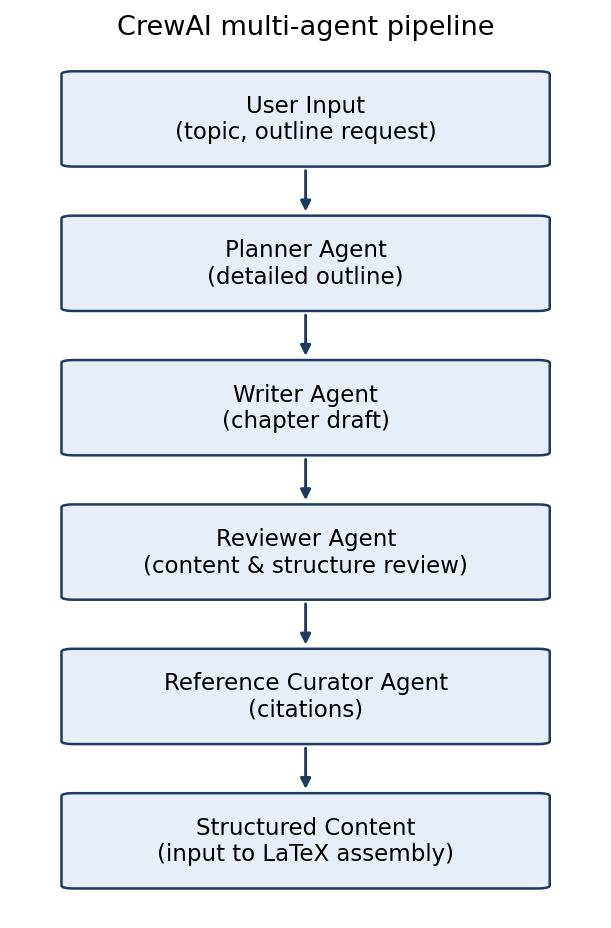
\includegraphics[width=0.75\textwidth]{figures/architecture.pdf}
%   \caption{Multi-agent pipeline architecture.}
%   \label{fig:architecture}
% \end{figure}

\section{Defining the Crew: Agent Roles and Responsibilities}
% TODO (Stage 9.3): content from book.md section 3.2 (four agent roles).

\section{Task Orchestration and Dependencies}
% TODO (Stage 9.3): content from book.md section 3.3 (sequential process).

% 04_implementation.tex — converted from content/book.md, "4. Implementation
% Details" (Stage 9.3). Code snippets use plain verbatim (no extra packages);
% citations mirror the [6]/[7] markers in the cleaned Markdown.

\chapter{Implementation Details}

\section{Agent Definitions and Personalities}

Each agent is created with a role, goal, and backstory. The example below
shows how an agent is configured in CrewAI. It uses the same model our real
run used, \texttt{gemini/gemini-2.5-flash}, rather than naming any specific
commercial product as a project result:

\begin{verbatim}
from crewai import Agent, LLM

llm = LLM(model="gemini/gemini-2.5-flash", temperature=0.2)

planner_agent = Agent(
    role="Content Planner",
    goal="Develop a clear, hierarchical outline for a technical LaTeX book.",
    backstory=(
        "You are an experienced technical editor. You break broad topics "
        "into logical chapters and sections and keep the table of contents "
        "coherent."
    ),
    llm=llm,
    verbose=True,
    allow_delegation=False,
)
\end{verbatim}

The writer, reviewer, and reference-curator agents follow the same pattern
with their own goals and backstories. The model is supplied from
configuration, and the API key is read from the environment only --- it is
never written into the source.

\section{Custom Tool Integration}

Tools extend agents beyond plain text generation. A realistic example for
this project is a \LaTeX{} validation tool that checks whether generated
\LaTeX{} compiles. The following is illustrative pseudocode for such a tool:

\begin{verbatim}
# latex_validation_tool.py (illustrative)
import subprocess
import tempfile
from pathlib import Path

def validate_latex(latex_code: str) -> str:
    """Attempt to compile a LaTeX snippet and report errors."""
    with tempfile.TemporaryDirectory() as tmp:
        tex = Path(tmp) / "snippet.tex"
        tex.write_text(
            "\\documentclass{article}\\begin{document}\n"
            f"{latex_code}\n\\end{{document}}\n",
            encoding="utf-8",
        )
        result = subprocess.run(
            ["pdflatex", "-interaction=nonstopmode",
             "-output-directory", tmp, str(tex)],
            capture_output=True,
            text=True,
        )
        if result.returncode == 0:
            return "Validation successful: no compilation errors."
        return "Validation failed: see compiler output for details."
\end{verbatim}

This shows the general idea of giving an agent a deterministic check it can
call. In the current project the deterministic checks live in plain Python
modules (for example the content-QA scanner) rather than being driven by the
LLM, which keeps the validation layer fully offline and reproducible.

\section{Task Design and Execution Flow}

Tasks are the atomic units of work. A simplified sequence for this project:

\begin{enumerate}
  \item \textbf{Plan outline} --- agent: planner; input: the topic; output:
        a structured outline.
  \item \textbf{Draft content} --- agent: writer; input: the outline;
        output: the draft.
  \item \textbf{Review} --- agent: reviewer; input: the draft; output:
        structured feedback.
  \item \textbf{Curate references} --- agent: reference curator; input:
        draft and review; output: the reference list.
\end{enumerate}

Table~\ref{tab:agents} summarises the agents, their roles, and example
tools.

\begin{table}[htbp]
  \centering
  \caption{Agents, roles, and example tools.}
  \label{tab:agents}
  \begin{tabular}{llll}
    \toprule
    Agent & Primary role & Example tasks & Example tools \\
    \midrule
    Planner & Structure the book & Outline generation, section split &
      OutlineTool \\
    Writer & Generate the prose & Drafting chapters and sections &
      WritingTool \\
    Reviewer & Quality assurance & Coverage and consistency checks &
      ReviewTool \\
    Reference curator & Collect citations & Building the reference list &
      ReferenceTool \\
    \bottomrule
  \end{tabular}
\end{table}

\section{Handling Multilingual Content}

The pipeline is designed to support content in more than one language, which
matters for documentation that mixes scripts. The relevant \LaTeX{} support
comes from packages such as \texttt{babel} or \texttt{polyglossia}, and for
bidirectional text the \texttt{bidi} package~\cite{ctan_bidi}, usually
compiled with XeLaTeX~\cite{tug_xetex} or LuaLaTeX for good Unicode and
right-to-left handling.

\paragraph{Hebrew--English bidirectional demonstration.} The following
passage demonstrates bidirectional typesetting: the text direction switches
automatically inside the right-to-left environment. This paragraph mixes
English and Hebrew text.

\begin{hebrew}
זוהי דוגמה למקטע הממחיש יצירת תוכן דו-לשוני.
\end{hebrew}

The English text flows left-to-right while the Hebrew sentence (meaning
``this is an example of a section demonstrating the creation of bilingual
content'') flows right-to-left, both within the same document ---
demonstrating correct bidirectional integration.

% 05_poc_to_production.tex — skeleton. Source: content/book.md,
% "5. From PoC to Production".
% TODO (Stage 9.3): transcribe sections 5.1-5.3 from content/book.md.

\chapter{From PoC to Production}

\section{Iterative Development and Refinement}
% TODO (Stage 9.3): content from book.md section 5.1.

\section{Deployment Considerations}
% TODO (Stage 9.3): content from book.md section 5.2.

\section{Monitoring, Maintenance, and CI/CD}
% TODO (Stage 9.3): content from book.md section 5.3.

% 06_results.tex — converted from content/book.md, "6. Results and
% Evaluation" (Stage 9.3). Measured values are exactly those in the cleaned
% Markdown (from the committed runtime.json); unmeasured metrics stay
% labelled as proposed. Citations mirror the [13]/[14] markers.

\chapter{Results and Evaluation}

\section{Generated LaTeX Examples}

The intended output of the full pipeline is structured content that converts
cleanly into \LaTeX{}. A representative chapter skeleton looks like this:

\begin{verbatim}
\chapter{Introduction to Multi-Agent Systems}
\label{ch:intro_mas}

\section{The Paradigm of Agentic AI}
\label{sec:agentic_ai}

Multi-agent systems distribute a complex task among specialised agents,
favouring modularity and robustness over a single monolithic model. In our
pipeline, each agent interprets its task, optionally uses tools, and passes
its output to the next agent in the sequence.
\end{verbatim}

This shows standard \verb|\chapter|, \verb|\section|, and \verb|\label|
structure with cross-referencing, which the \LaTeX{}-assembly stage produces
from the cleaned Markdown.

A numbered equation is included to satisfy the formula requirement. A simple
model for an agent's utility, balancing individual reward and collaboration,
is:

\begin{equation}
U_i(s, a_i) = R_i(s, a_i) + \alpha \sum_{j \neq i} C_{ij}(s, a_i, a_j)
\label{eq:agent_utility}
\end{equation}

where $U_i$ is the utility for agent $i$, $R_i$ its individual reward,
$C_{ij}$ the collaborative contribution from agent $j$, and $\alpha$ the
weight on collaboration.

\section{Measured Run and Proposed Metrics}

We report only what we actually measured. The figures below come directly
from the committed evidence of one real full run
(\texttt{results/stage8c7-full-gemini-20260611-173125/runtime.json})%
~\cite{mars777_runtime_evidence}, with the per-task breakdown recorded in the
crew output index of the same run~\cite{mars777_crew_index}. They describe a
single content-generation run, not an average over many books, and we do not
assert any monetary cost. Table~\ref{tab:measured-run} lists the measured
values.

\begin{table}[htbp]
  \centering
  \caption{Measured cost of the Stage 8C.7 full run.}
  \label{tab:measured-run}
  \begin{tabular}{lll}
    \toprule
    Metric & Value & Source \\
    \midrule
    Provider / model & gemini / \texttt{gemini/gemini-2.5-flash} &
      \texttt{runtime.json} \\
    Wall-clock runtime & 300.68 seconds &
      \texttt{runtime.json} (\texttt{elapsed\_seconds}) \\
    Prompt tokens & 213,664 &
      \texttt{runtime.json} (\texttt{prompt\_tokens}) \\
    Completion tokens & 235,436 &
      \texttt{runtime.json} (\texttt{completion\_tokens}) \\
    Agent/task calls & 4 (outline, draft, review, references) &
      \texttt{crew\_outputs/\_index.json} \\
    \bottomrule
  \end{tabular}
\end{table}

\paragraph{Proposed future evaluation metrics (not yet measured).} The
following would give a fuller picture of quality, but we have not run a
controlled study, so we report \emph{no numeric results} for them --- they
are proposals only:

\begin{itemize}
  \item generation time per chapter;
  \item a content-accuracy score from human and automated review;
  \item a structural-coherence score;
  \item a \LaTeX{} syntax-validity rate (fraction of generated files that
        compile cleanly).
\end{itemize}

Figure~\ref{fig:generation_time} is the Python-generated graph required by
the assignment. The script that produces it lives in
\texttt{scripts/generate\_graph.py}; its core is shown below. The values are
illustrative inputs for the chart, clearly labelled as such, not measured
results:

\begin{verbatim}
import matplotlib.pyplot as plt

# Illustrative example values for the figure (not measured results).
chapter_labels = ["Ch 1", "Ch 2", "Ch 3", "Ch 4", "Ch 5"]
example_times = [15, 20, 30, 45, 60]  # arbitrary illustrative minutes

plt.figure(figsize=(8, 5))
plt.bar(chapter_labels, example_times, color="steelblue")
plt.xlabel("Chapter")
plt.ylabel("Illustrative generation time (minutes)")
plt.title("Illustrative generation time per chapter")
plt.tight_layout()
plt.savefig("figures/generation_time.png", dpi=150)
\end{verbatim}

\begin{figure}[htbp]
  \centering
  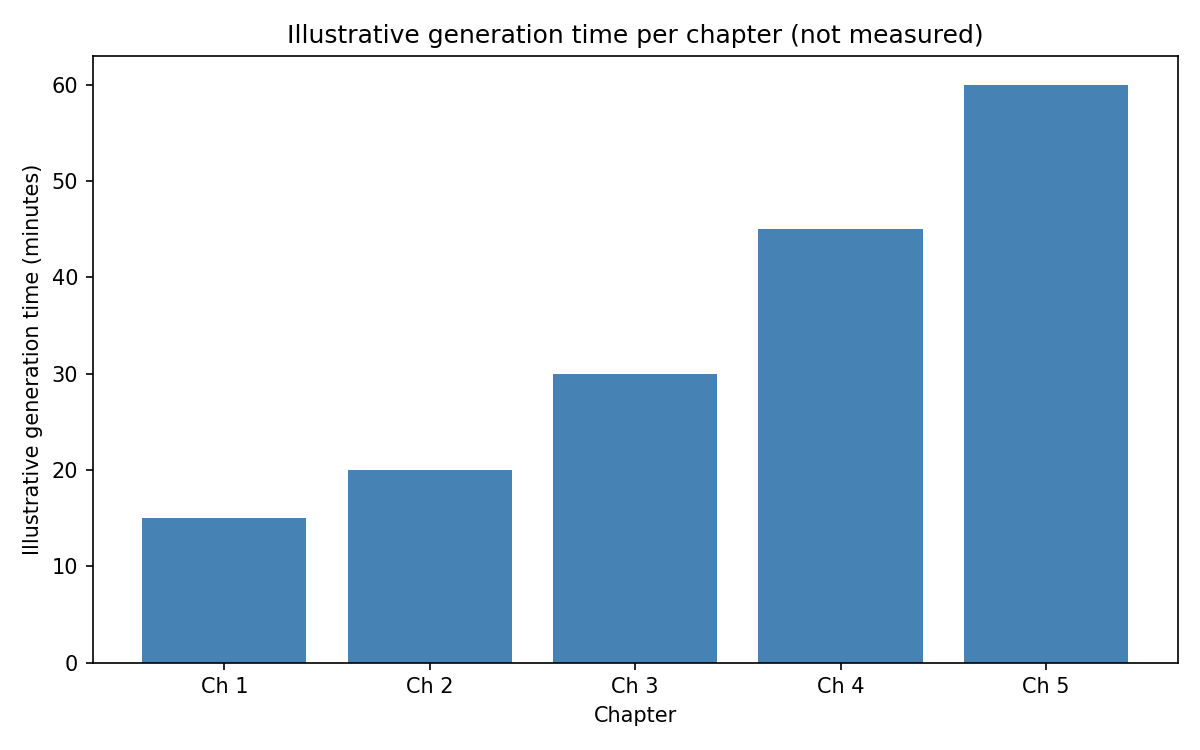
\includegraphics[width=0.8\textwidth]{figures/generation_time.png}
  \caption{Illustrative generation time per chapter (Python-generated).}
  \label{fig:generation_time}
\end{figure}

A weighted quality score gives a single comparable number once the component
scores exist. We define it but do not fill in fabricated values:

\begin{equation}
Q = w_A \cdot S_{A} + w_C \cdot S_{C} + w_F \cdot S_{F} + w_V \cdot S_{V}
\label{eq:quality}
\end{equation}

where $S_A, S_C, S_F, S_V$ are accuracy, coherence, formatting, and validity
sub-scores, and the non-negative weights satisfy $w_A + w_C + w_F + w_V = 1$.

\section{Qualitative Assessment}

From reading the generated drafts ourselves, the clear strengths are
structural consistency and fast first-draft generation: headings, sections,
and references come out uniformly, and a coherent draft appears quickly. The
clear weaknesses are limited depth on nuanced topics, no automatic generation
of complex graphics (figures are placeholders the assembler fills in), and
the need for human review before anything is considered final. This matches
our overall stance: the pipeline is a useful drafting assistant, not a
replacement for human judgement, and certainly not a finished production
system yet.

% 07_discussion.tex — skeleton. Source: content/book.md, "7. Discussion and
% Future Work".
% TODO (Stage 9.3): transcribe key findings, limitations, and future
% enhancements from content/book.md.

\chapter{Discussion and Future Work}
% TODO (Stage 9.3): content from book.md chapter 7.

% 08_conclusion.tex — converted from content/book.md, "8. Conclusion"
% (Stage 9.3).

\chapter{Conclusion}

This project designed, implemented, and partially evaluated a CrewAI
multi-agent pipeline for generating the content of a \LaTeX{} book. By
orchestrating a planner, writer, reviewer, and reference curator in a
sequential process --- and by keeping a separate deterministic layer for
validation --- the system produces structured, on-topic content from a
high-level topic. We measured the cost of one real run against
\texttt{gemini/gemini-2.5-flash} and reported it honestly, while clearly
labelling unmeasured metrics as proposals. The final article PDF was compiled
and validated locally, and the remaining work is submission packaging rather
than core pipeline construction. What we can claim is a working, inspectable
pipeline and an honest account of how it behaves.


% --- Bibliography (linked citations via biblatex/hyperref) -----------------
% The five project-internal docs entries are part of the cleaned bibliography
% (content/book.md entries 8-12) but are not cited in the body text; \nocite
% keeps them in the printed bibliography so it matches the cleaned source.
\nocite{mars777_prd,mars777_plan,mars777_quality,mars777_costs,mars777_decisions}
\printbibliography[heading=bibintoc,title={Bibliography}]

\end{document}
